\chapter{Series}
When writing a number with an infinite decimal, such as the Golden 
Ratio (also known as the Golden Number):
$$\phi = 1.618033988 \cdots$$

The decimal system means we can re-write the Golden Ratio (or any 
irrational number) as an infinite sum:
$$\phi = 1 + \frac{6}{10} + \frac{1}{10^2} + \frac{8}{10^3} + 
\frac{0}{10^4} + \frac{3}{10^5} + \cdots$$

You might recall from the chapter on Riemann Sums that we can 
represent the addition of many (or infinite) with big sigma notation:
$$\Sigma_{i = 1}^n a_i$$
Where i is the index as discussed in Sequences and n is the number of 
terms. For infinite sums, $n = \infty$.

\section{Partial Sums}
Let us quickly define a \textit{partial sum}. A partial sum is where 
we only look at the first $n$ terms of a series. For the general 
series, $\Sigma_{i=1}^{n} a_i$, the partial sums are:
$$s_1 = a_1$$
$$s_2 = a_1 + a_2$$
$$s_3 = a_1 + a_2 + a_3$$
$$\cdots$$
$$s_n = a_1 + a_2 + \cdots + a_n = \Sigma_{i=1}^{n} a_i$$

\textbf{Example}: A series is given by $\Sigma_{i=1}^\infty 
(\frac{-3}{4})^i$. What is the value of the partial sum $s_4$?

\textbf{Solution}: $s_4$ is the sum of the first 4 terms: 
$$(\frac{-3}{4})^1 + (\frac{-3}{4})^2 + (\frac{-3}{4})^3 + (\frac{-3}{4})^4$$
$$= \frac{-3}{4} + \frac{9}{16} + \frac{-27}{64} + \frac{81}{256} = \frac{-75}{256}$$


\section{Convergent and Divergent Series}
Just like sequences, series can also be convergent or divergent. 
Consider the series $\Sigma_{i=1}^\infty i$. Given what you already 
know about the meaning of "convergent" and "divergent", guess whether 
$\Sigma_{i=1}^\infty i$ is convergent or divergent. 

Let's determine the first few partial sums of the series (shown 
graphically in figure \ref{fig:divsum}):
\begin{center}
\begin{tabular}{|c|c|c|}\hline
n & Terms & Partial Sum\\
\hline
1 & 1 & 1\\
\hline
2 & 1+2 & 3\\
\hline
3 & 1+2+3 & 6\\
\hline
4 & 1+2+3+4 & 10\\
\hline
\end{tabular}
\end{center}

\begin{figure}[htbp]
\centering
    \begin{tikzpicture}
        \begin{axis}[axis lines = center, xmin = -0.5, xmax = 10, 
        ymin = 0, ymax = 55, xlabel=n, ylabel = $s_n$]
        \addplot[blue, mark=*](1,1);
        \addplot[blue, mark=*](2, 3);
        \addplot[blue, mark=*](3, 6);
        \addplot[blue, mark=*](4, 10);
        \addplot[blue, mark=*](5, 15);
        \addplot[blue, mark=*](6, 21);
        \addplot[blue, mark=*](7, 28);
        \addplot[blue, mark=*](8, 36);
        \addplot[blue, mark=*](9, 45);
        \addplot[blue, mark=*](10,55);
        \end{axis}
\end{tikzpicture}
    \caption{For the divergent series $\Sigma_{i=1}^n i$, the value of the 
    partial sum increases to infinity as $n$ increases}
    \label{fig:divsum}
\end{figure}

As you can see, as $n$ increases, the value of the partial sum 
increases without approaching a particular value. We can also see 
that the value of the first $n$ terms summed together is 
$\frac{n(n+1)}{2}$. This means that as $n$ approaches $\infty$, the 
sum also approaches $\infty$ and the series is divergent. 

Obviously, for a series to not become huge, the values of the terms 
should decrease as $i$ increases (that is, each subsequent term is 
smaller than the one before it). Take the series $\Sigma_{i=1}^\infty 
\frac{1}{2^i}$. As $i$ increases, $\frac{1}{2^i}$ decreases. Let's 
look at the first few partial sums of this series (shown graphically 
in figure \ref{fig:convsum}):
\begin{center}
\begin{tabular}{|c|c|c|}\hline
n & Terms & Partial Sum\\
\hline
1 & $\frac{1}{2}$ & $\frac{1}{2}$\\
\hline
2 & $\frac{1}{2} + \frac{1}{4}$ & $\frac{3}{4}$\\
\hline
3 & $\frac{1}{2} + \frac{1}{4} + \frac{1}{8}$ & $\frac{7}{8}$\\
\hline
4 & $\frac{1}{2} + \frac{1}{4} + \frac{1}{8} + \frac{1}{16}$ & 
$\frac{15}{16}$\\
\hline
\end{tabular}
\end{center}

\begin{figure}[htbp]
\centering
    \begin{tikzpicture}
        \begin{axis}[axis lines = center, xmin = -0.5, xmax = 8, 
        ymin = 0, ymax = 1.5, ytick = {1}, xlabel=n, ylabel = $s_n$]
        \addplot[blue, mark=*](1,0.5);
        \addplot[blue, mark=*](2, 3/4);
        \addplot[blue, mark=*](3, 7/8);
        \addplot[blue, mark=*](4, 15/16);
        \addplot[blue, mark=*](5, 31/32);
        \addplot[blue, mark=*](6, 63/64);
        \addplot[blue, mark=*](7, 127/128);
        \addplot[blue, mark=*](8, 255/256);
        \addplot[red, thin, dashed, domain = 0:8]{1};
        \end{axis}
\end{tikzpicture}
    \caption{For the convergent series $\Sigma_{i=1}^n \frac{1}{2^i}$, 
    the value of the partial sum approaches 1 as $n$ increases}
    \label{fig:convsum}
\end{figure}

Do you see the pattern? The $n^{th}$ partial sum is equal to 
$\frac{2^n - 1}{2^n} = 1 - \frac{1}{2^n}$. And as $n$ approaches 
$\infty$, the partial sum approaches 1. The series $\Sigma_{i=1}^\infty 
\frac{1}{2^i}$ is convergent. 

Let us define the sequence \{$s_n$\} where $s_n$ is the $n^{th}$ 
partial sum of a series:
$$s_n = \Sigma_{i=1}^n a_i$$. 

If the sequence \{$s_n$\} is convergent and $\lim_{n \to \infty} s_n$ 
exists, then the series $\Sigma_{i=1}^\infty a_i$ is also convergent. 
And if the sequence \{$s_n$\} is divergent, then the series 
$\Sigma_{i=1}^\infty a_i$ is also divergent.

\textbf{Example}: is the harmonic series, $\Sigma_{n = 1}^\infty \frac{1}{n}$ 
convergent or divergent?

\textbf{Solution}: You may think that the series is convergent, since $\lim_
{n \to \infty} \frac{1}{n} = 0$. Let's see if we can confirm this. We begin by 
looking at the partial sums $s_2$, $s_4$, $s_8$, and $s_16$:
$$s_2 = 1 + \frac{1}{2}$$
$$s_4 = 1 + \frac{1}{2} + \left(\frac{1}{3} + \frac{1}{4} \right) > 1 + 
\frac{1}{2} + \left( \frac{1}{4} + \frac{1}{4} \right) = 1 + \frac{2}{2}$$
$$s_8 = 1 + \frac{1}{2} + \left(\frac{1}{3} + \frac{1}{4} \right) + \left( 
\frac{1}{5} + \frac{1}{6} + \frac{1}{7} + \frac{1}{8} \right) > 1 + \frac{1}{2} 
+ \left(\frac{1}{4} + \frac{1}{4} \right) + \left( \frac{1}{8} + \frac{1}{8} + 
\frac{1}{8} + \frac{1}{8} \right) = 1 + \frac{3}{2}$$
$$s_{16} = 1 + \frac{1}{2} + \left(\frac{1}{3} + \frac{1}{4} \right) + \left( 
\frac{1}{5} + \frac{1}{6} + \frac{1}{7} + \frac{1}{8} \right) + \left(
\frac{1}{9} + \cdots + \frac{1}{16} \right) > $$
$$1 + \frac{1}{2} + \left(\frac{1}{4} + \frac{1}{4} \right) + \left( 
\frac{1}{8} + \frac{1}{8} + \frac{1}{8} + \frac{1}{8} \right) + \left(
\frac{1}{16} + \cdots + \frac{1}{16} \right) = 1 + \frac{4}{2}$$

Notice that, in general, $s_{2^n} > 1 + \frac{n}{2}$ for $n > 1$. Taking the 
limit as $n \to \infty$, we see that $\lim_{n \to \infty} s_{2^n} > \lim_{n 
\to \infty} 1 + \frac{n}{2} = \infty$. Therefore, $s_{2^n}$ also approaches 
$\infty$ as $n$ gets larger and the harmonic series $\Sigma_{n = 1}^\infty 
\frac{1}{n}$ is divergent. 

This example shows a very important point: the converse of a theorem is not 
always true! We do know that if a series is convergent, then the limit as n 
approaches infinity must be zero. The harmonic series shows that \textit{just 
because the limit as n approaches infinity is zero, the series is not 
necessarily convergent}. What we can say, though, is that the contrapositive 
statement is true: if the limit as n approaches infinity of a series does not 
exist or is not zero, then the series is divergent (i.e. not convergent). 

\subsection{Geometric Series}

Let's apply this definition of convergent and divergent to geometric 
series. You should recall from the chapter on sequences that a 
geometric sequence can be defined by $a_i = a(r)^{i-1}$, where $r$ 
is the common ratio and $a \neq 0$. We can express the 
\textit{geometric series} thusly:
$$a + ar + ar^2 + ar^3 = \Sigma_{i=1}^\infty ar^{i-1}$$

When are geometric series convergent? First, let's consider the case 
where $r=1$. If this is true, then $s_n = a + a + a + \cdots + a = 
na$. As $n$ approaches $\infty$, the sum will approach $\pm \infty$ 
(depending on whether $a$ is positive or negative), and the series is 
divergent. 

When $r \neq 1$, we can write $s_n$ and $rs_n$:
$$s_n = a + ar + ar^2 + \cdots + ar^{n-1}$$
$$rs_n = ar + ar^2 + ar^3 + \cdots + ar^n$$

Subtracting $rs_n$ from $s_n$, we get:
$$s_n - rs_n = (a + ar + ar^2 + \cdots + ar^{n-1}) - (ar + ar^2 + 
ar^3 + \cdots + ar^{n-1} + ar^n)$$
$$= a - ar^n$$

Solving for $s_n$, we find:
$$s_n = \frac{a(1-r^n)}{1-r}$$

We take the limit as $n \to \infty$ to determine for what values of 
$r$ the series converges:
$$\lim_{n \to \infty} s_n = \lim_{n \to \infty} \frac{a(1-r^n)}{1-r}$$
$$= \lim_{n\to \infty} \frac{a}{1-r} - \frac{ar^n}{1-r} = \frac{a}{1-r} 
- \frac{a}{1-r}\lim_{n \to \infty} r^n$$

This begs the question: when is $\lim_{n \to \infty} r^n$ convergent? 
From the sequences chapter, we know this limit converges if $|r| < 1$ 
(that is, $-1 < r < 1$). If this is true, then $\lim_{n \to \infty} 
r^n = 0$ and 
$$s_n = \frac{a}{1-r}$$

(see figures \ref{fig:geometric1} and \ref{fig:geometric2} for a visual)
\begin{figure}
    \centering
    \begin{tikzpicture}
        \begin{axis}[xmin = -0.5, xmax = 10, ymin = 0, axis lines = center, 
        xlabel = $n$, clip = false, ytick = \empty]
        \addplot[red, mark=*] (1, 2); %r=1.5
        \addplot[red, mark=*] (2, 5);
        \addplot[red, mark=*] (3, 19/2);
        \addplot[red, mark=*] (4, 65/4);
        \addplot[red, mark=*] (5, 211/8);
        \addplot[red, mark=*] (6, 665/16);
        \addplot[red, mark=*] (7, 2059/32);
        \node[red] at (5.5, 60) {$r > 1$};
        
        \addplot[orange, mark=*] (1, 2); %r=1
        \addplot[orange, mark=*] (2, 4);
        \addplot[orange, mark=*] (3, 6);
        \addplot[orange, mark=*] (4, 8);
        \addplot[orange, mark=*] (5, 10);
        \addplot[orange, mark=*] (6, 12);
        \addplot[orange, mark=*] (7, 14);
        \addplot[orange, mark=*] (8, 16);
        \addplot[orange, mark=*] (9, 18);
        \addplot[orange, mark=*] (10, 20);
        \node[orange] at (9, 25) {$r = 1$};
        
        \addplot[blue, mark =*] (1, 2); %r = 0.5
        \addplot[blue, mark =*] (2, 3);
        \addplot[blue, mark =*] (3, 7/2);
        \addplot[blue, mark =*] (4, 15/4);
        \addplot[blue, mark =*] (5, 31/8);  
        \addplot[blue, mark =*] (6, 63/16);
        \addplot[blue, mark =*] (7, 127/32);
        \addplot[blue, mark =*] (8, 255/64);
        \addplot[blue, mark =*] (9, 511/128);
        \addplot[blue, mark =*] (10, 1023/256);
        \node[blue] at (10, 10) {$0 < r < 1$};
        \end{axis}
    \end{tikzpicture}
    \caption{Geometric sequences are divergent if $r \geq 1$}
    \label{fig:geometric1}
\end{figure}

\begin{figure}
    \centering
    \begin{tikzpicture}
        \begin{axis}[xmin = -0.5, xmax = 10, axis lines = center, 
        xlabel = $n$, clip = false, ytick = \empty]
        \addplot[red, mark=*] (1, 2); %r=-1.5
        \addplot[red, mark=*] (2, -1);
        \addplot[red, mark=*] (3, 7/2);
        \addplot[red, mark=*] (4, -13/4);
        \addplot[red, mark=*] (5, 55/8);
        \addplot[red, mark=*] (6, -133/16);
        \addplot[red, mark=*] (7, 463/32);
        %\addplot[red, mark=*] (8, -1261/64);
        %\addplot[red, mark=*] (9, 4039/128);
        %\addplot[red, mark=*] (10, -11605/256);
        \node[red] at (5, 10) {$r > 1$};
        
        \addplot[orange, mark=*] (1, 2); %r=-1
        \addplot[orange, mark=*] (2, 0);
        \addplot[orange, mark=*] (3, 2);
        \addplot[orange, mark=*] (4, 0);
        \addplot[orange, mark=*] (5, 2);
        \addplot[orange, mark=*] (6, 0);
        \addplot[orange, mark=*] (7, 2);
        \addplot[orange, mark=*] (8, 0);
        \addplot[orange, mark=*] (9, 2);
        \addplot[orange, mark=*] (10, 0);
        \node[orange] at (9, -3) {$r = -1$};
        
        \addplot[blue, mark =*] (1, 2); %r = -0.5
        \addplot[blue, mark =*] (2, 1);
        \addplot[blue, mark =*] (3, 3/2);
        \addplot[blue, mark =*] (4, 5/4);
        \addplot[blue, mark =*] (5, 11/8);  
        \addplot[blue, mark =*] (6, 21/16);
        \addplot[blue, mark =*] (7, 43/32);
        \addplot[blue, mark =*] (8, 85/64);
        \addplot[blue, mark =*] (9, 171/128);
        \addplot[blue, mark =*] (10, 341/256);
        \node[blue] at (9, 5) {$-1 < r < 0$};
        \end{axis}
    \end{tikzpicture}
    \caption{Geometric sequences are divergent if $r \leq 1$. Notice that for 
    $r = -1$, the partial sums alternate between the initial term and zero.}
    \label{fig:geometric2}
\end{figure}

\textbf{Example}: Find the sum of the geometric series given by $2 - 
\frac{2}{3} + \frac{2}{9} - \frac{2}{27} + \cdots$. 

\textbf{Solution}: The first term is $a = 2$ and each the common 
ratio is $r = \frac{-1}{3}$. Since $|r| < 1$, we know that the series 
converges. We can calculate the value of the sum using the geometric 
series formula: 
$$\Sigma_{i=1}^\infty a(r)^{i-1} = \frac{a}{1-r}$$
$$\Sigma_{i=1}^\infty 2(\frac{-1}{3})^{i-1} = \frac{2}{1-\frac{-1}{3}} = 
\frac{2}{\frac{4}{3}} = \frac{6}{4} = 1.5$$

We can confirm this graphically (see figure \ref{fig:geometric}). You 
can also write out the first several partial sequences: you should 
find the sums approach 1.5 as $n$ increases.

\begin{figure}[htbp]
\centering
    \begin{tikzpicture}
        \begin{axis}[axis lines = center, xmin = -0.5, xmax = 8, 
        ymin = -1.5, ymax = 2, xlabel=n, legend pos = south east]
        \addplot[blue, mark=*](1,2);
        \addlegendentry{$s_n$};
        \addplot[red, mark=o](1, 2);
        \addlegendentry{$a_n$};
        \addplot[blue, mark=*](2, 4/3);
        \addplot[blue, mark=*](3, 14/9);
        \addplot[blue, mark=*](4, 40/27);
        \addplot[blue, mark=*](5, 122/81);
        \addplot[blue, mark=*](6, 364/243);
        \addplot[blue, mark=*](7, 1094/729);
        \addplot[blue, mark=*](8, 3280/ 2187);
        \addplot[red, mark=o](2, -2/3);
        \addplot[red, mark=o](3, 2/9);
        \addplot[red, mark=o](4, -2/27);
        \addplot[red, mark=o](5, 2/81);
        \addplot[red, mark=o](6, -2/243);
        \addplot[red, mark=o](7, 2/729);
        \addplot[red, mark=o](8, -2/2187);
        \addplot[red, thin, dashed, domain = 0:8]{1.5};
        \end{axis}
\end{tikzpicture}
    \caption{the $n^{th}$ term and partial sums of $\Sigma_{i=1}^n 
    2(\frac{-1}{3})^{i-1}$}
    \label{fig:geometric}
\end{figure}

\section{The Integral Test}
We were able to determine the exact value of some infinite series because it 
was possible to write the $n^{th}$ partial sum, $s_n$, in terms of $n$. For 
example, we determined that the $n^{th}$ partial sum of $\Sigma_{i = 1}^n 
\frac{1}{2^i}$ is $s_n = 1 - \frac{1}{2^n}$. However, it is not always possible 
to do this. How can we estimate the value of an infinite series in cases where 
we can't explicitly write $s_n$ in terms of $n$?

Consider the series $\Sigma_{i = 1}^\infty \frac{1}{i^2}$. The first few terms 
are:
$$\Sigma_{i = 1}^\infty \frac{1}{2^i} = \frac{1}{1^2} + \frac{1}{2^2} + 
\frac{1}{3^2} + \frac{1}{4^2} + \frac{1}{5^2} + \cdots$$

The series is decreasing, but is it convergent? Let's plot this series on an 
$xy$-plane (see figure \ref{fig:invsquare1}). 

\begin{figure}[htbp]
    \centering
    \begin{tikzpicture}
        \begin{axis}[xmin = -0.25, xmax = 6, axis lines = center, xlabel = $n$, 
        ymin = 0, ymax = 1.25, ytick = \empty]
        \foreach \n in {1,...,5}{
        \addplot[red, mark=*]({\n}, {1/(\n)^2});
        }
        \end{axis}
    \end{tikzpicture}
    \caption{The first 5 terms of $\Sigma_{i = 1}^\infty \frac{1}{2^i}$}
    \label{fig:invsquare1}
\end{figure}

We can overlay the function $y = \frac{1}{2^x}$ (figure \ref{fig:invsquare2}). 
We can draw rectangles of width 1 and height $\frac{1}{x^2}$ (see figure 
\ref{fig:invsquare3}). The area of the first $n$ rectangles is equal to the 
$n^{th}$ partial sum. 

\begin{figure}[htbp]
    \centering
    \begin{tikzpicture}
        \begin{axis}[xmin = -0.25, xmax = 6, axis lines = center, 
        xlabel = $n$, ymin = 0, ymax = 1.25, ytick = \empty]
        \foreach \n in {1,...,5}{
        \addplot[red, mark=*]({\n}, {1/(\n)^2});
        }
        \addplot[blue, domain = 0.7:6] {1/x^2};
        \end{axis}
    \end{tikzpicture}
    \caption{The first 5 terms of $\Sigma_{i = 1}^\infty \frac{1}{2^i}$ lie on 
    the curve $y = \frac{1}{x^2}$}
    \label{fig:invsquare2}
\end{figure}

\begin{figure}[htbp]
    \centering
    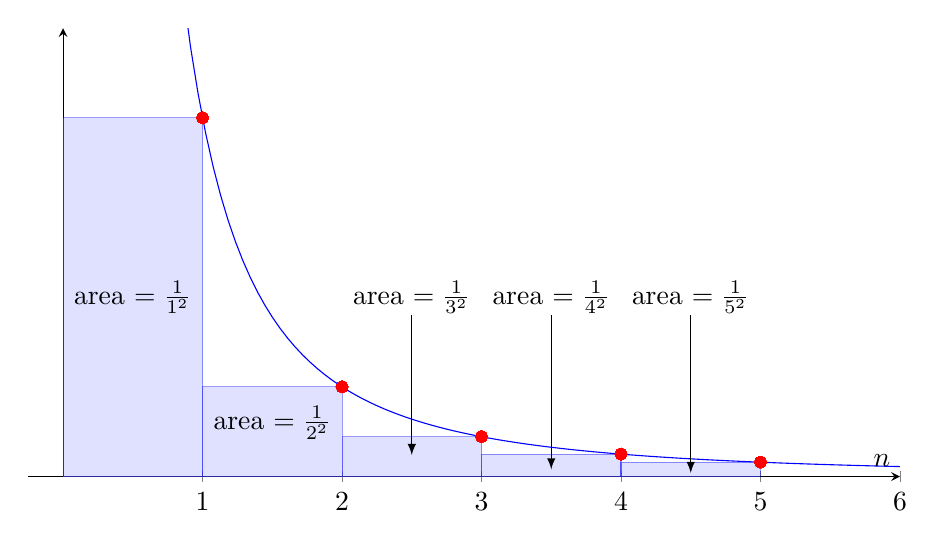
\begin{tikzpicture}
        \begin{axis}[xmin = -0.25, xmax = 6, axis lines = center, xlabel = $n$, 
        ymin = 0, ymax = 1.25, ytick = \empty, width = 1.5*\axisdefaultwidth, 
        height = \axisdefaultheight]
        \foreach \n in {1,...,5}{
        \addplot[red, mark=*]({\n}, {1/(\n)^2});
        }
        \addplot[blue, domain = 0.7:6, samples=100] {1/x^2};
        \filldraw[fill=blue!30, draw = blue, opacity = 0.4] 
        (0, 0) rectangle (1,  1);
        \filldraw[fill=blue!30, draw = blue, opacity = 0.4] 
        (1, 0) rectangle (2, 0.25);
        \filldraw[fill=blue!30, draw = blue, opacity = 0.4] 
        (2, 0) rectangle (3,  1/9);
        \filldraw[fill=blue!30, draw = blue, opacity = 0.4] 
        (3, 0) rectangle (4,  1/16);
        \filldraw[fill=blue!30, draw = blue, opacity = 0.4] 
        (4, 0) rectangle (5,  1/25);
        \node[] at (0.5, 0.5) {area $=\frac{1}{1^2}$};
        \node[] at (1.5, 0.15) {area $=\frac{1}{2^2}$};
        \node[] at (2.5, 0.5) {area $=\frac{1}{3^2}$};
        \node[] at (3.5, 0.5) {area $=\frac{1}{4^2}$};
        \node[] at (4.5, 0.5) {area $=\frac{1}{5^2}$};
        \draw[-latex](2.5, 0.45) -- (2.5, 0.06);
        \draw[-latex](3.5, 0.45) -- (3.5, 0.02);
        \draw[-latex](4.5, 0.45) -- (4.5, 0.01);
        \end{axis}
    \end{tikzpicture}
    \caption{The $5^{th}$ partial sum of $\Sigma_{i=1}^\infty \frac{1}{2^i}$ 
    is equal to the area of the rectangles}
    \label{fig:invsquare3}
\end{figure}

This should remind you of a Riemann sum. Since the total area of the rectangles 
is less than the area under the curve, we can state:
$$\Sigma_{i = 1}^\infty \frac{1}{2^i} < \int_0^\infty \frac{1}{x^2}\,dx$$

We can exclude the first rectangle and also state that: 
$$\Sigma_{i = 1}^\infty \frac{1}{2^i}< 1 + \int_1^\infty \frac{1}{x^2}\,dx$$

We can evaluate this integral:
$$\int_1^\infty \frac{1}{x^2}\,dx = \lim_{t \to \infty} \left[ \int_1^t 
\frac{1}{x^2}\,dx \right]$$
$$ = \lim_{t \to \infty} \frac{-1}{x}|_{x=1}^t = \lim_{t \to \infty} \left( 
\frac{-1}{t} \right) - \frac{-1}{1} = 0 - (-1) = 1$$

And therefore:
$$\Sigma_{i = 1}^\infty \frac{1}{2^i}< 1 + 1 = 2$$

This means the series $\Sigma_{i = 1}^\infty \frac{1}{2^i}$ is bounded above. 
Since the series is also monotonic (each term is positive, so the value of the 
sum increases as $n$ increases), we can state that the sum is convergent! 

Let's look at a divergent example: $\Sigma_{i = 1}^\infty \frac{1}{\sqrt{x}}$. 
Again, we will make a visual, but this time we will draw rectangles that lie 
above the curve $y = \frac{1}{\sqrt{x}}$ (see figure \ref{fig:invroot}). In 
this case, $\Sigma_{i = 1}^\infty \frac{1}{\sqrt{x}}> \int_1^\infty 
\frac{1}{\sqrt{x}}\,dx$. Let's evaluate the integral:
$$\int_1^\infty \frac{1}{\sqrt{x}}\,dx = \lim_{t \to \infty} \left[ \int_1^t 
\frac{1}{\sqrt{x}}\,dx \right] $$
$$= \lim_{t \to \infty} \left[ 2 \sqrt{x} \right]_{x=1}^t= \lim_{t \to \infty} 
\left( 2\sqrt{t} \right) - 2\sqrt{1} = \infty - 2 \rightarrow \text{divergent}$$

Since the integral diverges to infinity and the series is greater than the 
integral, the series must also diverge to infinity. This is another case where 
a monotonic decreasing series is not convergent!

\begin{figure}[htbp]
    \centering
    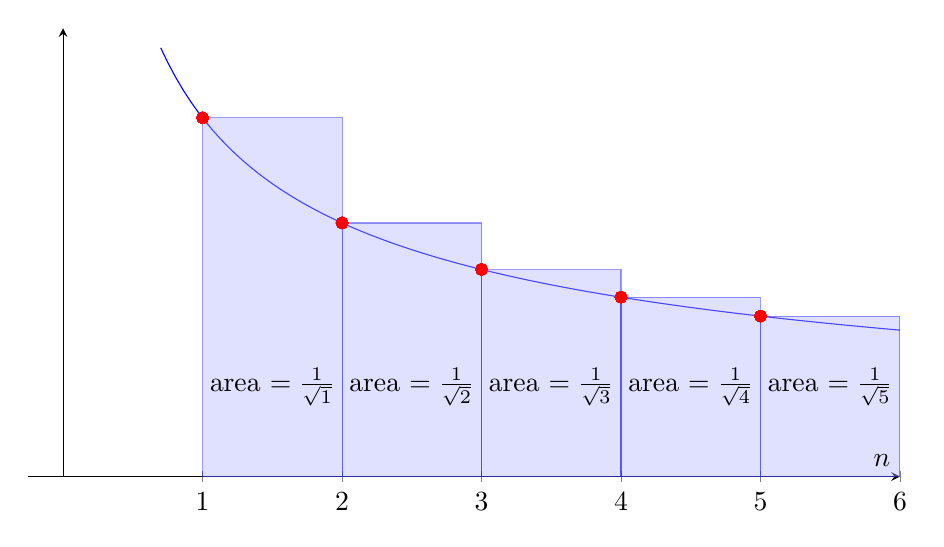
\begin{tikzpicture}
        \begin{axis}[xmin = -0.25, xmax = 6, axis lines = center, xlabel = $n$, 
        ymin = 0, ymax = 1.25, ytick = \empty, width = 1.5*\axisdefaultwidth, 
        height = \axisdefaultheight]
        \foreach \n in {1,...,5}{
        \addplot[red, mark=*]({\n}, {1/sqrt(\n)});
        }
        \addplot[blue, domain = 0.7:6, samples=100] {1/sqrt(x)};
        \filldraw[fill=blue!30, draw = blue, opacity = 0.4] 
        (1, 0) rectangle (2,  1);
        \filldraw[fill=blue!30, draw = blue, opacity = 0.4] 
        (2, 0) rectangle (3, 0.707);
        \filldraw[fill=blue!30, draw = blue, opacity = 0.4] 
        (3, 0) rectangle (4,  0.577);
        \filldraw[fill=blue!30, draw = blue, opacity = 0.4] 
        (4, 0) rectangle (5,  0.5);
        \filldraw[fill=blue!30, draw = blue, opacity = 0.4] 
        (5, 0) rectangle (6, 0.4472);
        \node[] at (1.5, 0.25) {area $=\frac{1}{\sqrt{1}}$};
        \node[] at (2.5, 0.25) {area $=\frac{1}{\sqrt{2}}$};
        \node[] at (3.5, 0.25) {area $=\frac{1}{\sqrt{3}}$};
        \node[] at (4.5, 0.25) {area $=\frac{1}{\sqrt{4}}$};
        \node[] at (5.5, 0.25) {area $=\frac{1}{\sqrt{5}}$};
        \end{axis}
    \end{tikzpicture}
    \caption{$\Sigma_{i = 1}^\infty \frac{1}{\sqrt{x}}> \int_1^\infty 
    \frac{1}{\sqrt{x}}\,dx$}
    \label{fig:invroot}
\end{figure}

This leads us to the \textbf{Integral Test}. If $f$ is a continuous, positive, 
decreasing function on the interval $x \in [1, \infty)$ and $a_n = f(n)$, then 
the series $\Sigma_{n=1}^\infty a_n$ converges if and only if $\int_1^\infty 
f(x)\,dx$ is convergent. Subsequently, if $\int_1^\infty f(x)\,dx$ is 
divergent, then the series is also divergent.

\textbf{Example}: Is the series $\Sigma_{i = 1}^\infty \frac{1}{n^2 + 1}$ 
convergent or divergent?

\textbf{Solution}: To apply the integral test, we define $f(x) = 
\frac{1}{x^2 + 1}$, which is a positive, decreasing function on the interval 
$x \in [1, \infty)$. 
$$\int_1^\infty \frac{1}{x^2 + 1}\,dx = \lim_{t \to \infty} \int_{1}^t 
\frac{1}{x^2 + 1}\,dx$$
$$= \lim_{t \to \infty} \left[ \arctan{x} \right]_{x = 1}^t = \lim_{t \to \infty} 
\left( \arctan{t} \right) - \arctan{1} = \frac{\pi}{2} - \frac{\pi}{4} = 
\frac{\pi}{4}$$

Because the integral $\int_1^\infty \frac{1}{x^2 + 1}\,dx$ converges, so does 
the series $\Sigma_{n = 1}^\infty \frac{1}{n^2 + 1}$. 

\begin{Exercise}[label = series1]
Use the integral test to determine if the following series are convergent or 
divergent. 
\begin{enumerate}
\item $\Sigma_{n = 1}^\infty 2n^{-3}$
\item $\Sigma_{n = 1}^\infty \frac{5}{3n-1}$
\item $\Sigma_{n = 1}^\infty \frac{n}{3n^2 + 1}$
\end{enumerate}
\vspace{40mm}
\end{Exercise}

\begin{Answer}[ref= series1]
\begin{enumerate}
\item The function $2x^{-3}$ is positive and decreasing for $x \in [1, \infty)$. 
$\int_1^\infty 2x^{-3}\,dx = \lim_{t \to \infty} \int_1^t 2x^{-3}\,dx = \lim_{t 
\to \infty} \left[-x^{-2} \right]_{x = 1}^t = \lim_{t \to \infty} ( -t^{-2}) - 
-(1)^{-2} = 0 + 1 = 1$. Since the integral $\int_1^\infty 2x^{-3}\,dx$ converges, 
the series $\Sigma_{n = 1}^\infty 2n^{-3}$ is also convergent.
\item The function $\frac{5}{3x+1}$ is positive and decreasing for $x \in [1, 
\infty)$. $\int_1^\infty \frac{5}{3x-1}\,dx = \lim_{t \to \infty} \int_1^t 
\frac{5}{3x-1}\,dx$ Using u-substitution to evaluate the integral, we set $u = 
3x-1$ and find that $du = 3dx \rightarrow dx = \frac{du}{3}$. Substituting, 
$\int_1^t \frac{5}{3x-1}\,dx = \int_{x=1}^{x=t} \frac{5}{3}\frac{1}{u}\,du$. 
Evaluating the integral, $\int_{x=1}^{x=t} \frac{5}{3}\frac{1}{u}\,du = 
\frac{5}{3}\ln{u}|_{x = 1}^{x =t} = \frac{5}{3}\ln{3x+1}|_{1}^t$. Substituting 
this back into the limit, $\int_1^\infty \frac{5}{3x-1}\,dx = \lim_{t \to 
\infty} \frac{5}{3}\ln{3x+1}|_{1}^t = \lim_{t \to \infty} [ \frac{5}{3} 
\ln{3t+1} ] - \frac{5}{3}\ln{4} = \infty - \frac{5}{3}\ln{4} = \infty$. 
Therefore, the integral $\int_1^\infty \frac{5}{3x-1}\,dx$ is divergent and so 
is the series $\Sigma_{n = 1}^\infty \frac{5}{3n-1}$
\item The function $\frac{x}{3x^2 + 1}$ is positive and decreasing for $x\in 
[1,\infty)$. $\int_1^\infty \frac{x}{3x^2 + 1}\,dx = \lim_{t \to \infty} 
\int_1^t \frac{x}{3x^2 + 1}\,dx$. Applying the substitution $u = 3x^2 + 1$ 
and $\frac{du}{6} = x\text{ }dx$, we see that $\lim_{t \to \infty} \int_1^t 
\frac{x}{3x^2 + 1}\,dx = \lim_{t \to \infty} \int_{x=1}^{x=t} \frac{1}{6u}\,du 
= \lim_{t \to \infty} \frac{1}{6}\ln{u}|_{x = 1}^{x = t} = \lim_{t \to \infty} 
\frac{1}{6}\ln{3x^2 + 1}|_{1}^{t} = \lim_{t \to \infty} \left[ \frac{1}{6}
\ln{3t^2 + 1} \right] - \frac{1}{6}\ln{4} = \infty$. Therefore the integral 
$\int_1^\infty \frac{x}{3x^2 + 1}\,dx$ is divergent and so is the series 
$\Sigma_{n = 1}^\infty \frac{n}{3n^2 + 1}$. 
\end{enumerate}
\end{Answer}

\subsection{p-series}
A $p$-series takes the form $\Sigma_{n=1}^\infty \frac{1}{n^p}$. For what 
values of $p$ does the $p$-series converge? We can apply the integral test to 
find a general rule. First, we consider $p < 0$. 
Since $p < 0$, we will define $q = -p$ and note that $q > 0$. Then $\Sigma_
{n=1}^\infty \frac{1}{n^p} = \Sigma_{n=1}^\infty n^q$. And we can see that:
$$\lim_{n \to \infty}\frac{1}{n^p} = \lim_{n \to \infty}n^q$$
Since $q > 0$, $\lim_{n \to \infty}n^q = \infty$. Since $a_n$ does not 
approach zero as $n \to \infty$, we know that $\Sigma_{n = 1}^\infty 
\frac{1}{n^p}$ diverges for $p < 0$. 

Next we examine the case where $p=0$. Since any real number raised to zero 
power is 1, we can see that $lim_{n \to \infty} \frac{1}{n^p} = \lim_{n \to 
\infty} 1 = 1$. Again, since $a_n$ does not approach zero as $n \to \infty$, 
the series diverges for $p = 0$. 

When $p > 0$, the function $f(x) = \frac{1}{x^p}$ is continuous, positive, and 
decreasing on the interval $[1, \infty)$ and we can apply the integral test to 
determine if $\Sigma_{n=1}^\infty \frac{1}{n^p}$ converges or diverges. We 
already know that $\int_1^\infty \frac{1}{x}\,dx = \lim_{x \to \infty} \ln{x} 
= \infty$. Since the integral diverges when $p = 1$, then the series $\Sigma_
{n=1}^\infty \frac{1}{x^p}$ also diverges for $p = 1$. 

When $p > 0$ and $p \neq 1$, then:
$$\int_1^\infty \frac{1}{x^p}\,dx = \lim_{t \to \infty} \int_1^t x^{-p}\,dx $$
$$= \lim_{t \to \infty} \frac{x^{-p + 1}}{-p + 1}|_{x=1}^{x=t} = \left( \frac{1}
{1 - p} \right) \lim_{t \to \infty} \left( \frac{1}{t^{p - 1}} - 1 \right)$$

If $p > 1$, then $p - 1 >0$ and $\lim_{t \to \infty} \frac{1}{t^{p - 1}} = 
\frac{1}{\infty} = 0$ and the integral $\int_1^\infty \frac{1}{x^p}\,dx$ 
converges to $\frac{1}{p - 1}$. 

If $p < 1$, then $1 - p > 0$ and $\lim_{t \to \infty} \frac{1}{t^{p - 1}} = 
\lim_{t \to \infty} t^{1 - p} = \infty$ and the integral $\int_1^\infty 
\frac{1}{x^p}\,dx$ diverges. 

So, in summary, the $p$-series $\Sigma_{n = 1} ^ \infty \frac{1}{x^p}$ converges 
if $p > 1$ and diverges if $p \leq 1$. 

\subsection{Using Integrals to Estimate the Value of a Series}
Recall that $\Sigma_{i=1}^\infty a_i = a_1 + a_2 + a_3 + \cdots = s$ and that 
the $n^{th}$ partial sum, often represented as $s_n$, is $s_n = a_1 + a_2 + 
\cdots + a_{n-1} + a_n$. Then we can define the $n^{th}$ remainder $R_n = s - 
s_n$. Expanding $s$ and $s_n$, we see that:
$$R_n = \left[ a_1 + a_2 + \cdots + a_{n-1} + a_n + a_{n+1} + \cdots \right] - 
\left[ a_1 + a_2 + \cdots + a_{n-1} + a_{n} \right]$$
$$R_n = [a_1 - a_1] + [a_2 - a_2] + \cdots + [a_{n-1} - a_{n-1}] + [a_n - a_n] 
+ a_{n-1} + a_{n-2} + \cdots$$
$$R_n = a_{n+1} + a_{n+2} + a_{n+3} + \cdots$$

Just like the integral test, suppose there is some continuous, positive, 
decreasing function such that $a_n = f(n)$. The we can represent $R_n$ as the 
right Riemann sum with width $\Delta x = 1$ from $x = n$ to $\infty$. Since 
the rectangles are below the curve (see figure \ref{fig:remainderceiling}), we 
can state that $R_n \leq \int_n^\infty f(x)\,dx$.

\begin{figure}[htbp]
    \centering
    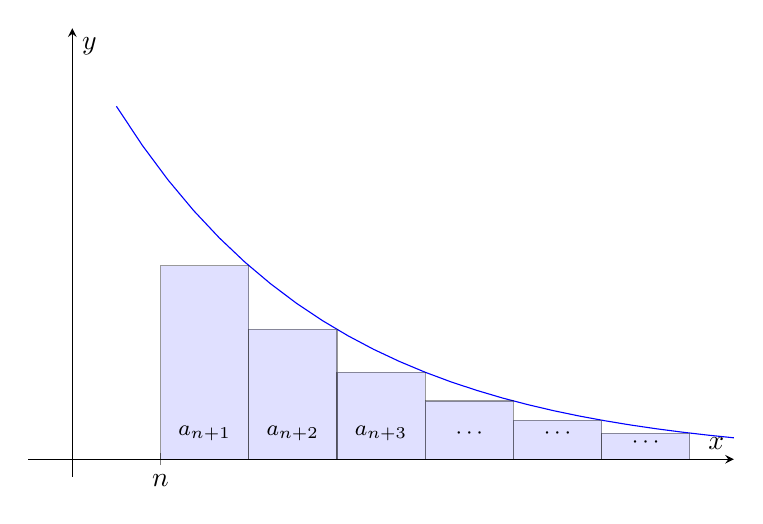
\begin{tikzpicture}
        \begin{axis}[xmin = -0.1, xmax = 1.5, axis lines = center, 
        xlabel = $x$, ymin = -0.2, ymax = 5, ytick = \empty, 
        width = 1.25*\axisdefaultwidth, height = \axisdefaultheight, 
        xtick={0.2}, xticklabels={$n$}, ylabel={$y$}]
        \addplot[blue, domain = 0.1:1.5]{5*e^(-2*x)};
        \filldraw[fill=blue!30, draw=black, opacity = 0.4] 
        (0.2, 0) rectangle (0.4, {5*e^(-2*0.4)});
        \filldraw[fill=blue!30, draw=black, opacity = 0.4] 
        (0.4, 0) rectangle (0.6, {5*e^(-2*0.6)});
        \filldraw[fill=blue!30, draw=black, opacity = 0.4] 
        (0.6, 0) rectangle (0.8, {5*e^(-2*0.8)});
        \filldraw[fill=blue!30, draw=black, opacity = 0.4] 
        (0.8, 0) rectangle (1, {5*e^(-2*1)});
        \filldraw[fill=blue!30, draw=black, opacity = 0.4] 
        (1, 0) rectangle (1.2, {5*e^(-2*1.2)});
        \filldraw[fill=blue!30, draw=black, opacity = 0.4] 
        (1.2, 0) rectangle (1.4, {5*e^(-2*1.4)});
        \node[font=\footnotesize] at (0.3, 0.3) {$a_{n+1}$};
        \node[font=\footnotesize] at (0.5, 0.3) {$a_{n+2}$};
        \node[font=\footnotesize] at (0.7, 0.3) {$a_{n+3}$};
        \node[font=\footnotesize] at (0.9, 0.3) {$\cdots$};
        \node[font=\footnotesize] at (1.1, 0.3) {$\cdots$};
        \node[font=\footnotesize] at (1.3, 0.2) {$\cdots$};
        \end{axis}
    \end{tikzpicture}
    \caption{$R_n \leq \int_n^\infty f(x)\,dx$ }
    \label{fig:remainderceiling}
\end{figure}

Similarly, we can represent $R_n$ as the left Riemann sum with width $\Delta x 
= 1$ from $x= n + 1$ to $\infty$. This time the rectangles are above the curve 
(see figure \ref{fig:remainderfloor}), and we can state that $R_n \geq \int_
{n+1}^\infty f(x)\,dx$. Putting this all together, we have an estimate for the 
remainder, $R_n$, from the integral test:

Suppose there is a function such that $f(k) = a_k$, where $f$ is a continuous, 
positive, decreasing function for $x \geq n$ and $\Sigma a_n$ is convergent. 
Then, $\int_{n+1}^\infty f(x)\,dx \leq R_n \leq \int_N^\infty f(x)\,dx$, where 
$R_n$ is the $s - s_n$. 

\begin{figure}[htbp]
    \centering
    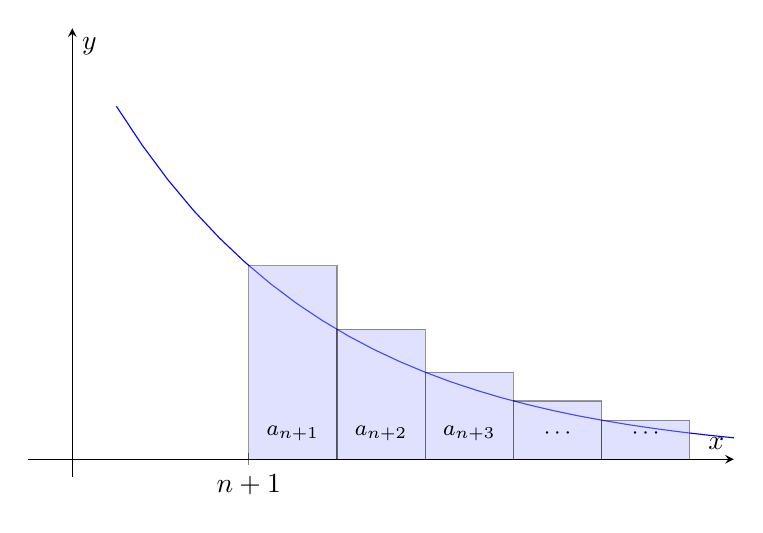
\begin{tikzpicture}
        \begin{axis}[xmin = -0.1, xmax = 1.5, axis lines = center, 
        xlabel = $x$, ymin = -0.2, ymax = 5, ytick = \empty, 
        width = 1.25*\axisdefaultwidth, height = \axisdefaultheight, 
        xtick={0.4}, xticklabels={$n+1$}, ylabel={$y$}]
        \addplot[blue, domain = 0.1:1.5]{5*e^(-2*x)};
        \filldraw[fill=blue!30, draw=black, opacity = 0.4] 
        (0.4, 0) rectangle (0.6, {5*e^(-2*0.4)});
        \filldraw[fill=blue!30, draw=black, opacity = 0.4] 
        (0.6, 0) rectangle (0.8, {5*e^(-2*0.6)});
        \filldraw[fill=blue!30, draw=black, opacity = 0.4] 
        (0.8, 0) rectangle (1, {5*e^(-2*0.8)});
        \filldraw[fill=blue!30, draw=black, opacity = 0.4] 
        (1, 0) rectangle (1.2, {5*e^(-2*1)});
        \filldraw[fill=blue!30, draw=black, opacity = 0.4] 
        (1.2, 0) rectangle (1.4, {5*e^(-2*1.2)});
        \node[font=\footnotesize] at (0.5, 0.3) {$a_{n+1}$};
        \node[font=\footnotesize] at (0.7, 0.3) {$a_{n+2}$};
        \node[font=\footnotesize] at (0.9, 0.3) {$a_{n+3}$};
        \node[font=\footnotesize] at (1.1, 0.3) {$\cdots$};
        \node[font=\footnotesize] at (1.3, 0.3) {$\cdots$};
        \end{axis}
    \end{tikzpicture}
    \caption{$R_n \geq \int_{n+1}^\infty f(x)\,dx$ }
    \label{fig:remainderfloor}
\end{figure}

\textbf{Example}: Approximate the sum of the series $\Sigma_{n=1}^\infty 
\frac{3}{n^3}$ by finding the $10^{th}$ partial sum. Estimate the error of 
this approximation. 

\textbf{Solution}: Using a calculator, you can find the $10^{th}$ partial sum: 
$$\Sigma_{n=1}^{10} \frac{3}{n^3} = \frac{3}{1^3} + \frac{3}{2^3} + 
\frac{3}{3^3} + \cdots + \frac{3}{10^3} \approx 3.593 = s_{10}$$

Recall that the remainder, $R_{10}$ is the difference between the actual sum, 
$s$, and the partial sum, $s_{10}$. Using the integral test to estimate the 
remainder, we can state that: $$R_{10} \leq \int_{10}^\infty \frac{3}{x^3}\,dx 
= \frac{3}{2(10)^2} = \frac{3}{200} = 0.015$$ Therefore, the size of the error 
is at most 0.015. 

\textbf{Example}: How many terms are required for the error to be less than 
0.0001?

\textbf{Solution}: We are looking for an $n$ such that $R_n \leq 0.0001$. 
Recalling that $R_n \leq \int_{n}^\infty \frac{3}{x^3}\,dx$, we need to find 
an $n$ such that $\int_{n}^\infty \frac{3}{x^3}\,dx \leq 0.0001$. 

$$\int_n^\infty \frac{3}{x^3}\,dx \leq 0.0001$$
$$\frac{-1}{6x^2}|_{x=n}^\infty \leq 0.0001$$
$$\lim_{x \to \infty} \frac{-1}{6x^2} - \frac{-1}{6n^2} \leq 0.0001$$
$$0 + \frac{1}{6n^2} = \frac{1}{6n^2} \leq 0.0001$$
$$1 \leq 0.0006n^2$$
$$1667 \leq n^2$$
$$40.8 \leq n \rightarrow n = 41$$
Therefore, $s - s_{41} \leq 0.0001$ and the partial sum $\Sigma_{n=1}^{41} 
\frac{3}{n^3}$ is less than 0.0001 from the value of the infinite sum $\Sigma_
{n=1}^\infty \frac{3}{n^3}$.

\begin{Exercise}[label=remainder1]
\begin{enumerate}
\item Find the partial sum $s_{10}$ of the series $\Sigma_{n=1}^\infty 
\frac{1}{n^4}$. 
\item Estimate the error from using $s_{10}$ as an approximation of the series.
\item Use $s_n + \int_{n+1}^\infty \frac{1}{x^4}\,dx \leq s \leq s_n + \int_n^
\infty \frac{1}{x^4}\,dx$ to give an improved estimate of the sum.
\item The actual value of $\Sigma_{n=1}^\infty \frac{1}{n^4}$ is 
$\frac{\pi^4}{90}$. Compare your estimate with the actual value.
\item Find a value of $n$ such that $s_n$ is within 0.00001 of the sum. 
\end{enumerate}
\vspace{50mm}
\end{Exercise}

\begin{Answer}[ref=remainder1]
\begin{enumerate}
\item $s_{10} = \frac{1}{1^4} + \frac{1}{2^4} + \cdots + \frac{1}{10^4} \approx 
1.082037$. 
\item $R_{10} \leq \int_{10}^\infty \frac{1}{x^4}\,dx = \frac{-1}{3x^3}|_
{x=10}^\infty = \lim_{x \to \infty} \frac{-1}{3x^3} - \frac{-1}{3 \cdot 10^3} 
= \frac{1}{3000} = 0.000333$. Therefore, the error is less than 0.000333. 
\item Given $s_{10} \approx 1.082037$, we can say that $1.082037 + \int_{n+1}^
\infty \frac{1}{x^4}\,dx \leq s \leq 1.082037 + \int_{n}^{\infty} \frac{1}{x^4}
\,dx$. Using a calculator to evaluate each integral, we see that: $1.082037 + 
0.000250 \leq s \leq 1.082037 + 0.000333$ and therefore the sum is between 
1.082287 and 1.082370. 
\item Writing the actual value as a decimal, $\frac{\pi^4}{90} \approx 
1.082323$, which is in the estimate window from the previous part. 
\item We are looking for an $n$ such that $\int_n^\infty \frac{1}{x^4}\,dx 
\leq 0.00001$. $\lim_{x \to \infty} \frac{-1}{3x^3} - \frac{-1}{3n^3} = 
\frac{1}{3n^3} \leq 0.00001$. $100,000 \leq 3n^3$. $33,333.33 \leq n^3$. 
$32.183 \leq n$. Since $n$ must be an integer, $n=33$ gives $R_n \leq 0.00001$. 
\end{enumerate}
\end{Answer}

\section{Comparison Tests}
In comparison tests, we compare a series to a known convergent or divergent 
series. Take the series $\Sigma_{n=1}^\infty \frac{1}{3^n + 3}$. This is 
similar to $\Sigma_{n=1}^\infty \frac{1}{3^n}$, which is a geometric series 
that converges to $\frac{1}{2}$. Notice that:
$$\frac{1}{3^n + 3} < \frac{1}{3^n}$$
Which implies that 
$$\Sigma_{n=1}^\infty \frac{1}{3^n + 3} < \Sigma_{n=1}^\infty \frac{1}{3^n}$$

Since $\Sigma_{n=1}^\infty \frac{1}{3^n}$ is convergent, it follows that 
$\Sigma_{n=1}^\infty \frac{1}{3^n + 3}$ is also convergent (see figure 
\ref{fig:compare1}). As you can see, since  $\Sigma_{n=1}^\infty \frac{1}{3^n}$ 
approaches $\frac{1}{2}$, $\Sigma_{n=1}^\infty \frac{1}{3^n + 3}$ must be $\leq 
\frac{1}{2}$ and therefore convergent. 

\begin{figure}
    \centering
    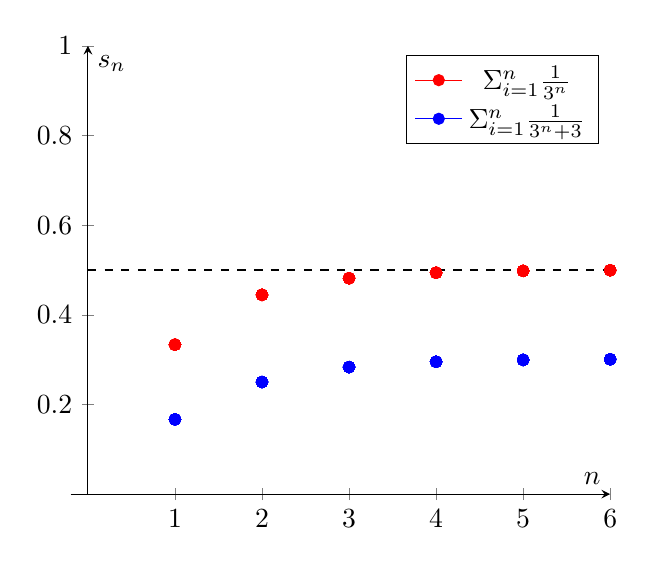
\begin{tikzpicture}
        \begin{axis}[xmin=-0.2, xmax = 6, ymin = 0, ymax=1, 
        axis lines = center, xlabel=$n$, ylabel = $s_n$]
        \addplot[red, mark=*](1, 1/3);
        \addlegendentry{$\Sigma_{i=1}^n \frac{1}{3^n}$};
        \addplot[blue, mark=*](1, 1/6);
        \addlegendentry{$\Sigma_{i=1}^n \frac{1}{3^n+3}$};
        \addplot[red, mark=*](2, 4/9);
        \addplot[red, mark=*](3, 13/27);
        \addplot[red, mark=*](4, 40/81);
        \addplot[red, mark=*](5, 121/243);
        \addplot[red, mark=*](6, 364/729);
        \addplot[blue, mark=*](2, 1/4);
        \addplot[blue, mark=*](3, 17/60);
        \addplot[blue, mark=*](4, 31/105);
        \addplot[blue, mark=*](5, 859/2870);
        \addplot[blue, mark=*](6, 315829/1050420);
        \addplot[black, dashed, domain = 0:6]{0.5};
        \end{axis}
    \end{tikzpicture}
    \caption{$\Sigma_{i=1}^n \frac{1}{3^n + 3} < \Sigma_{i = 1}^n 
    \frac{1}{3^n}$ for all $n$}
    \label{fig:compare1}
\end{figure}
\subsection{The Direct Comparison Test}
For the \textbf{Direct Comparison Test}, we compare the terms $a_n$ to $b_n$ 
directly. Take $\Sigma a_n$ and $\Sigma b_n$ to be series with positive terms. 
Then, 
\begin{enumerate}
\item If $a_n \leq b_n$ and $\Sigma b_n$ is convergent, then $\Sigma a_n$ is 
also convergent.
\item If $a_n \geq b_n$ and $\Sigma b_n$ is divergent, then $\Sigma a_n$ is 
also divergent.
\end{enumerate}

We already discussed why the first part is true above. The second part follows 
a similar argument: if $a_n$ is greater than $b_n$, then you can imagine that 
as $\Sigma b_n$ grows and diverges, it is pushing upwards on $\Sigma a_n$, 
meaning that $\Sigma a_n$ must also diverge. Consider the series $\Sigma_{n=1}^
\infty \frac{2\ln{n}}{n}$. For $n \geq 2$, $2\ln{n} > 1$, and therefore if 
$\Sigma_{n=1}^\infty \frac{1}{n}$ diverges, then $\Sigma_{n=1}^\infty \frac{2
\ln{n}}{n}$ must also diverge. We recognize the harmonic series $\Sigma_{n=1}^
\infty \frac{1}{n}$ is divergent. Therefore, $\Sigma_{n=1}^\infty 
\frac{2\ln{n}}{n}$ is also divergent (see figure \ref{fig:compare2}).

\begin{figure}
    \centering
    \begin{tikzpicture}
        \begin{axis}[xmin=-0.2, xmax = 8, ymin = 0, axis lines = center, 
        xlabel=$n$, ylabel = $s_n$, legend style={at={(0.45,1)}}]
        \addplot[red, mark=*, only marks] coordinates {(1, 1) (2, 3/2) 
        (3, 11/6) (4, 25/12) (5, 137/60) (6, 49/20) (7, 363/140) (8, 761/280)};
        \addlegendentry{$\Sigma_{i=1}^n \frac{1}{n}$};
        \addplot[blue, mark=*, only marks] coordinates {(1, 0) (2, 0.693) 
        (3, 1.426) (4, 2.119) (5, 2.762) (6, 3.360) (7, 3.916) (8, 4.436)};
        \addlegendentry{$\Sigma_{i=1}^n \frac{2\ln{n}}{n}$};
        \end{axis}
    \end{tikzpicture}
    \caption{$\Sigma_{i=1}^n \frac{2\ln{n}}{n} > \Sigma_{i=1}^n \frac{1}{n}$ 
    for $n \geq 4$}
    \label{fig:compare2}
\end{figure}

\subsection{The Limit Comparison Test}
Consider the series $\Sigma_{n=1}^\infty \frac{1}{2^n - 1}$. We may want to compare this to the convergent series $\Sigma_{n=1}^\infty \frac{1}{2^n}$. The direct comparison test isn't helpful here, since $\frac{1}{2^n - 1} > \frac{1}{2^n}$, so $\Sigma_{n=1}^\infty \frac{1}{2^n}$ doesn't put a cap on $\Sigma_{n=1}^\infty \frac{1}{2^n - 1}$ like our earlier example (see figure \ref{fig:compare1}). In a case such as this, we can use the \textbf{Limit Comparison Test}, which states that:
If $\Sigma a_n$ and $\Sigma b_n$ are series with positive terms and $\lim_{n \to \infty} \frac{a_n}{b_n} = c > 0$, then either both series converge or both series diverge.

Let's apply this to the series $\Sigma_{n=1}^\infty \frac{1}{2^n - 1}$. We know that $\Sigma_{n=1}^\infty \frac{1}{2^n}$ converges, since it is a geometric series with $r < 1$. 
$$\lim_{n \to \infty} \frac{\frac{1}{2^n - 1}}{\frac{1}{2^n}} = \lim_{n \to \infty} \frac{1}{2^n - 1} \cdot \frac{2^n}{1}$$
$$= \lim_{n \to \infty} \frac{2^n}{2^n - 1} = \lim_{n \to \infty} \frac{1}{1-1/2^n} = \frac{1}{1-0} = 1 > 0$$

Therefore, by the Limit comparison test, $\Sigma_{n=1}^\infty \frac{1}{2^n - 1}$ converges.

In general, comparison tests are most useful for series resembling geometric or $p$-series. When choosing a $p$-series to compare the unknown series to, choose $p$ such that the order of your $p$ series is the same as the order of the unknown series.

\textbf{Example}: What $p$-series should one compare the series $\Sigma_{n=1}^\infty \frac{\sqrt{n^3 + 1}}{3n^3 + 4n^2 + 2}$ to?

\textbf{Solution}: We can determine the order of $\frac{\sqrt{n^3 + 1}}{3n^3 + 4n^2 + 2}$ by looking at the highest-order terms in the numerator and denominator:
$$\frac{\sqrt{n^3}}{n^3} = \frac{n^{3/2}}{n^3} = \frac{1}{n^{3/2}}$$
So we should compare $\Sigma_{n=1}^\infty \frac{\sqrt{n^3 + 1}}{3n^3 + 4n^2 + 2}$ to the convergent $p$-series $\Sigma_{n=1}^\infty \frac{1}{n^{3/2}}$.

\begin{Exercise}[label = comp1]
Use the Comparison Test or the Limit Comparison Test to determine if the following series are convergent or divergent. 
\begin{enumerate}
\item $\Sigma_{n=1}^\infty \frac{1}{\sqrt{n^2 + 1}}$
\item $\Sigma_{n=1}^\infty \frac{9^n}{3 + 10^n}$
\item $\Sigma_{n=1}^\infty \frac{n \sin^2{n}}{1 + n^3}$
\end{enumerate}
\end{Exercise}

\begin{Answer}[ref = comp1]
\begin{enumerate}
\item This is similar to $\Sigma_{n=1}^\infty \frac{1}{n}$, which is divergent. Unfortunately, $\frac{1}{n} > \frac{1}{\sqrt{n^2 + 1}}$, so we can't use the 
direct comparison test. We will try the limit comparison test:
$$\lim_{n \to \infty} \left( \frac{\frac{1}{\sqrt{n^2 + 1}}}{\frac{1}{n}} 
\right) = \lim_{n \to \infty} \left( \frac{1}{\sqrt{n^2 + 1}} \cdot \frac{n}{1} 
\right) = \lim_{n \to \infty} \frac{n}{\sqrt{n^2 + 1}} = \lim_{n \to \infty} 
\frac{1}{\sqrt{1 + 1/n^2}} = \frac{1}{1+ 0} = 1 > 0$$
Therefore, since $\Sigma_{n=1}^\infty \frac{1}{n}$ diverges, so does $\Sigma_
{n=1}^\infty \frac{1}{\sqrt{n^2 + 1}}$.
\item This series is similar to the convergent geometric series $\Sigma_{n=1}^
\infty \left( \frac{9}{10} \right)^n$. Given that:
$$\left( \frac{9}{10} \right) = \frac{9^n}{10^n} < \frac{9^n}{3 + 10^n}$$
Since $\frac{9^n}{3 + 10^n} < \left( \frac{9}{10} \right)^n$ and $\Sigma_{n=1}
^\infty \left( \frac{9}{10} \right)^n$ is convergent, by the direct comparison 
test, $\Sigma_{n=1}^\infty \frac{9^n}{3 + 10^n}$ is also convergent. 
\item We can compare this to the convergent $p$-series $\Sigma_{n=1}^\infty \frac{1}{n^2}$. Noting that $\sin^2{n} \leq 1$:
$$\frac{n \sin^2{n}}{1 + n^3} < \frac{n \sin^2{n}}{n^3} \leq \frac{n}{n^3} = \frac{1}{n^2}$$
Because $\frac{n \sin^2{n}}{1 + n^3} \leq \frac{1}{n^2}$ for all $n \geq 1$ and $\Sigma_{n=1}^\infty \frac{1}{n^2}$ is convergent, we can state by the direct comparison test that $\Sigma_{n=1}^\infty \frac{n \sin^2{n}}{1 + n^3}$ is also convergent. 
\end{enumerate}
\end{Answer}

\section{Alternating Series}
FIXME write alternating series section
\section{Ratio and Root Tests for Convergence}
\subsection{Absolute Convergence}
Suppose there is a series $\Sigma_{n=1}^\infty a_n$, then there is a 
corresponding series $\Sigma_{n=1}^\infty |a_n| = |a_1| + |a_2| + |a_3| + 
\cdots$. If $\Sigma_{n=1}^\infty |a_n|$ is convergent, then the series $\Sigma_
{n=1}^\infty a_n$ is called \textbf{absolutely convergent}. 

\textbf{Example}: Consider the alternating series 
$$\Sigma_{n=1}^\infty \frac{(-1)^{n-1}}{n^2} = 1 - \frac{1}{2^2} + 
\frac{1}{3^2} + \cdots$$\\
Is this series absolutely convergent?

\textbf{Solution}: We examine the corresponding series where we take the 
absolute value of each term:
$$\Sigma_{n=1}^\infty \left|\frac{(-1)^{n-1}}{n^2} \right| = \Sigma_{n=1}^
\infty \frac{1}{n^2}$$
We can identify $\Sigma_{n=1}^\infty \frac{1}{n^2}$ as a convergent $p$-series. 
Since $\Sigma_{n=1}^\infty \frac{1}{n^2}$ is convergent, we can state that 
$\Sigma_{n=1}^\infty \frac{(-1)^{n-1}}{n^2}$ is absolutely convergent. 

\textbf{Example} Is the convergent series $\Sigma_{n=1}^\infty 
\frac{(-1)^{n-1}}{n}$ absolutely convergent?

\textbf{Solution} We consider the sum of the absolute values of the terms:
$$\Sigma_{n=1}^\infty \left|\frac{(-1)^{n-1}}{n}\right| = \Sigma_{n=1}^\infty 
\frac{1}{n}$$\\
You should recognize this as the harmonic series, which is divergent. When a 
series is convergent but the corresponding series of absolute values is not, 
we call it \textbf{conditionally convergent}. 

We won't prove the theorem here, but it is useful to know that if a series 
$\Sigma_{n=1}^\infty a_n$ is absolutely convergent, then it is convergent. You 
can prove this yourself using the Comparison Test. 

\begin{Exercise}[label = absconv1]
Is the series given by 
$$\frac{\cos{1}}{1^2} + \frac{\cos{2}}{2^2} + \frac{\cos{3}}{3^3} + \cdots$$ \\
convergent or divergent?
\vspace{40mm}
\end{Exercise}

\begin{Answer}[ref = absconv1]
We can write the series as $\Sigma_{n=1}^\infty \frac{\cos{n}}{n^2}$. Since 
$n$ is real, we know that $n^2 > 0$ and we can say that $\Sigma_{n=1}^\infty 
\left| \frac{\cos{n}}{n^2} \right| = \Sigma_{n=1}^\infty \frac{|\cos{n}|}
{n^2}$. Additionally, $|\cos{n}| \leq 1$ for all $n$, and therefore 
$\frac{|\cos{n}|}{n^2} \leq \frac{1}{n^2}$. We know the series $\Sigma_{n=1}^
\infty \frac{1}{n^2}$ is convergent. And since we have shown that $\Sigma_{n=1}
^\infty \frac{|\cos{n}|}{n^2} \leq \Sigma_{n=1}^\infty \frac{1}{n^2}$, by the 
comparison test $\Sigma_{n=1}^\infty \frac{|\cos{n}|}{n^2}$ is convergent. 
Therefore, $\Sigma_{n=1}^\infty \frac{\cos{n}}{n^2}$ is absolutely convergent 
and therefore convergent. 
\end{Answer}

\begin{Exercise}[label = absconv2]
Determine whether each of the following series is absolutely or conditionally 
convergent. 
\begin{enumerate}
\item $\Sigma_{n=1}^\infty \frac{(-1)^n}{3n + 2}$
\item $\Sigma_{n=1}^\infty \frac{\sin{n}}{4^n}$
\item $\Sigma_{n=1}^\infty (-1)^{n-1} \frac{2n}{n^2-4}$ 
\end{enumerate}
\vspace{50mm}
\end{Exercise}

\begin{Answer}[ref = absconv2]
\begin{enumerate}
\item $\Sigma_{n=1}^\infty \left| \frac{(-1)^n}{3n+2} \right| = \Sigma_{n=1}^
\infty \frac{1}{3n + 2}$ Applying the integral test to this sum: $\int_1^
\infty \frac{1}{3x+2}\,dx = \lim_{t \to \infty} \int_1^t \frac{1}{3x+2}\,dx = 
\left[ \frac{1}{3} \ln{3x + 2} \right]_{x=1}^t = \lim_{t \to \infty} \left[ 
\ln{3x + 2} \right] - \ln{3(1) - 2} = \infty - 0 = \infty$. Since $\int_1^\infty 
\frac{1}{3x + 2}\,dx$ is divergent, $\Sigma_{n=1}^\infty \frac{1}{3n + 2}$ is 
divergent and $\Sigma_{n=1}^\infty \frac{(-1)^n}{3n + 2}$ is conditionally 
convergent.
\item $\Sigma_{n=1}^\infty \left| \frac{\sin{n}}{4^n} \right| \leq \Sigma_{n=1}
^\infty \frac{1}{4^n}$. Applying the integral test to $\Sigma_{n=1}^\infty 
\frac{1}{4^n}$: $\int_1^\infty \frac{1}{4^x}\,dx = \lim_{t \to \infty} 
\frac{-1}{4^x \ln{4}}|_{x=1}^t = \lim_{t \to \infty} \left[ \frac{-1}{4^t 
\ln{4}} \right] - \frac{-1}{4^1 \ln{4}} = 0 + \frac{1}{4 \ln{4}} = \frac{1}{4 
\ln{4}}$. Since $\int_1^\infty \frac{1}{4^x}\,dx$ is convergent, the series 
$\Sigma_{n=1}^\infty \frac{1}{4^n}$ is also convergent. And since $\Sigma_{n=1}
^\infty \left| \frac{\sin{n}}{4^n} \right| \leq \Sigma_{n=1}^\infty 
\frac{1}{4^n}$, $\Sigma_{n=1}^\infty \left| \frac{\sin{n}}{4^n} \right|$ is 
also convergent, which shows that $\Sigma_{n=1}^\infty \frac{\sin{n}}{4^n}$ is 
absolutely convergent. 
\end{enumerate}
\end{Answer}

\subsection{The Ratio Test}
The ratio test compares the $(n + 1)^{th}$ term of a series to the $n^{th}$ term 
and takes the limit as $n \to \infty$ of the absolute value of this ratio:
$$\lim_{n \to \infty} \left| \frac{a_{n + 1}}{a_n} \right| = L$$
There are three possible outcomes of the ratio test:
\begin{enumerate}
\item if $L < 1$, then the series $\Sigma_{n=1}^\infty a_n$ is absolutely 
convergent (and therefore convergent).
\item if $L = 1$, then the ratio test is inconclusive and we cannot draw any 
conclusions about whether $\Sigma_{n=1}^\infty a_n$ is convergent or divergent.
\item if $L > 1$ or $\lim_{n \to \infty} \frac{a_{n + 1}}{a_n} = \infty$, then 
the series $\Sigma_{n=1}^\infty a_n$ is divergent.
\end{enumerate}

\textbf{Example}: Apply the ratio test to determine if $\Sigma_{n=1}^\infty 
(-1)^n \frac{n^3}{3^n}$.

\textbf{Solution}: 
$$\lim_{n \to \infty} \left| \frac{\frac{(-1)^{n + 1}(n + 1)^3}{3^{n + 1}}}{
\frac{(-1)^n n^3}{3^n}} \right| = \lim_{n \to \infty} \frac{(n + 1)^3}{3^{n + 
1}} \cdot \frac{3^n}{n^3}$$
$$= \lim_{n \to \infty} \frac{(n + 1)^3}{n^3} \cdot \frac{3^n}{3 \cdot 3^n}$$
$$= \lim_{n \to \infty} \left( \frac{n + 1}{n} \right) \cdot \frac{1}{3} = 
\frac{1}{3} \lim_{n \to \infty} \left( \frac{n + 1}{n} \right) = \frac{1}{3} 
\cdot 1 = \frac{1}{3} $$
Since $L < 1$, the series $\Sigma_{n=1}^\infty (-1)^n \frac{n^3}{3^n}$ is absolutely convergent. 

The ratio test is most useful for series that contain factorials, constants raised to the $n^{th}$ power, or other products. 

\begin{Exercise}[label = ratio1]
[This question was originally presented as a multiple-choice, no-calculator problem on the 2012 AP Calculus BC exam.] Which of the following series are convergent?
\begin{enumerate}
\item $\Sigma_{n=1}^\infty \frac{8^n}{n!}$
\item $\Sigma_{n=1}^\infty \frac{n!}{n^{100}}$
\item $\Sigma_{n=1}^\infty \frac{n + 1}{(n)(n+2)(n+3)}$
\end{enumerate}
\end{Exercise}

\begin{Answer}[ref = ratio1]
Series 1 and 3 converge
\begin{enumerate}
\item We apply the ratio test: $\lim_{n \to \infty} \left| \frac{\frac{8^
{n + 1}}{(n + 1)!}}{\frac{8^n}{n!}} \right| = \lim_{n \to \infty} \frac{8 
\cdot 8^n}{(n + 1)(n!)} \cdot \frac{n!}{8^n} = \lim_{n \to \infty} 
\frac{8}{n + 1} = 0$. Therefore, the series converges. 
\item We apply the ratio test: $\lim_{n \to \infty} \left| \frac{\frac{(n + 1)!}
{(n + 1)^{100}}}{\frac{n!}{n^{100}}} \right| = \lim_{n \to \infty} \frac{(n + 1)
n!}{(n + 1)^{100}} \cdot \frac{n^{100}}{n!} = \lim_{n \to \infty} \left( 
\frac{n}{n + 1} \right)^{100} \cdot (n + 1) = \lim_{n \to \infty} \frac{n^{100}
}{(n + 1)^{99}} = \infty$. Therefore, the series diverges. 
\item We apply the comparison test: $\frac{n + 1}{(n)(n + 2)(n + 3)} = \frac{n}
{(n)(n + 2)(n + 3)} + \frac{1}{(n)(n + 2)(n + 3)} = \frac{1}{(n + 2)(n + 3)} + 
\frac{1}{(n)(n + 2)(n + 3)} = \frac{1}{n^2 + 5n + 6} + \frac{1}{n^3 + 5n^2 + 
6n} \leq \frac{1}{n^2} + \frac{1}{n^3}$. The series $\Sigma_{n = 1}^\infty 
\frac{1}{n^2}$ and $\Sigma_{n = 1}^\infty \frac{1}{n^3}$ are both convergent, 
because they are $p$-series with $p > 1$. Having established that $\Sigma_{n=1}
^\infty \frac{n + 1}{(n)(n + 2)(n + 3)} \leq \Sigma_{n=1}^\infty \frac{1}{n^2} 
+ \frac{1}{n^3}$ and that $\Sigma_{n=1}^\infty \frac{1}{n^2} + \frac{1}{n^3}$ 
converges, by the comparison test we can state that $\Sigma_{n=1}^\infty 
\frac{n + 1}{(n)(n+2)(n+3)}$ converges. 
\end{enumerate}
\end{Answer}

\begin{Exercise}[label = series2]
[This question was originally presented as a multiple-choice, calculator-allowed 
problem on the 2012 AP Calculus BC exam.]If the series $\Sigma_{n = 1}^\infty 
a_n$ converges and $a_n > 0$ for all $n$, which of the following statements 
must be true? Explain. 
\begin{enumerate}
\item $\lim_{n \to \infty} \left| \frac{a_{n + 1}}{a_n} \right| = 0$
\item $|a_n|<1$ for all $n$
\item $\Sigma_{n=1}^\infty a_n = 0$
\item $\Sigma_{n=1}^\infty na_n$ diverges
\item $\Sigma_{n=1}^\infty \frac{a_n}{n}$ converges
\end{enumerate}
\end{Exercise}

\begin{Answer}[ref=label2]
\begin{enumerate}
\item This is not necessarily true. For a convergent series, the result of the 
ratio test is $L < 1$, so the limit could be $\neq 0$. 
\item This is not necessarily true. Consider the geometric series $\Sigma_{n=1}
^\infty 2(\frac{1}{2})^{n-1}$. This series is convergent because the common 
ratio is less than one, but the first term is $2(\frac{1}{2})^0 = 2 > 1$. 
\item This is not necessarily true. Again, consider the geometric series 
$\Sigma_{n=1}^\infty 2(\frac{1}{2})^{n-1}$, which converges to $4 \neq 0$. 
\item This is not necessarily true. Consider the $p$-series $\Sigma_{n=1}^
\infty \frac{1}{n^4}$. Then the series $\Sigma_{n=1}^\infty n \frac{1}{n^4} = 
\Sigma_{n=1}^\infty \frac{1}{n^3}$ is convergent. 
\item This must be true. By the comparison test, $\Sigma_{n=1}^\infty 
\frac{a_n}{n} \leq \Sigma_{n = 1}^\infty a_n$. Since $\Sigma_{n = 1}^\infty 
a_n$ converges, so much $\Sigma_{n = 1}^\infty na_n$. 
\end{enumerate}
\end{Answer}

\subsection{Root Test}
The root test examines the behavior of the $n^{th}$ root of $a_n$ as $n \to 
\infty$. Similar to the ratio test, there are three possible outcomes:
\begin{enumerate}
\item If $\lim_{n \to \infty} \sqrt[n]{|a_n|} = L < 1$, then the series $\Sigma
_{n=1}^\infty a_n$ is absolutely convergent, and therefore convergent.
\item If $\lim_{n \to \infty} \sqrt[n]{|a_n|} = L >1$ or $\lim_{n \to \infty} 
\sqrt[n]{|a_n|} = \infty$, then the series $\Sigma_{n=1}^\infty a_n$ is 
divergent.
\item If $\lim_{n \to \infty} \sqrt[n]{|a_n|} = L = 1$, then the Root Test is 
inconclusive. 
\end{enumerate}

The root test is best when there is a term or terms raised to the $n^{th}$ 
power. Consider the series $\Sigma_{n=1}^\infty \left( \frac{2n + 3}{3n + 2} 
\right)^n$:

\textbf{Example}: Is the series $\Sigma_{n=1}^\infty \left( \frac{2n + 3}{3n + 
2} \right)^n$ convergent or divergent?

\textbf{Solution}: Since $a_n$ consists of terms raised to the $n^{th}$ power, 
we will apply the root test for convergence:
$$\lim_{n \to \infty} \sqrt[n]{\left| \left( \frac{2n+3}{3n+2} \right)^n 
\right|} = \lim_{n \to \infty} \frac{2n+3}{3n+2} = \frac{2}{3} < 1$$ 
Therefore, by the root test, the series $\Sigma_{n=1}^\infty \left( \frac{2n + 
3}{3n + 2} \right)^n$ is convergent. 

\begin{Exercise}[label=root1]
Use the Root Test to determine whether the following series are convergent or 
divergent.
\begin{enumerate}
\item $\Sigma_{n=1}^\infty \left( \frac{3n^2 + 1}{n^2 - 4} \right)^n$
\item $\Sigma_{n=1}^\infty \frac{(-1)^{n}}{(\ln{n})^n}$
\item $\Sigma_{n=1}^\infty \left( 1+ \frac{1}{n} \right)^{n^2}$
\end{enumerate}
\end{Exercise}

\begin{Answer}
\begin{enumerate}
\item $\lim_{n=1}^\infty \sqrt[n]{\left| \left( \frac{3n^2 + 1}{n^2 - 4} \right)^n 
\right|} = \lim_{n=1}^\infty \frac{3n^2 + 1}{n^2 - 4} = 3 >1$. Therefore, 
the series $\Sigma_{n=1}^\infty \left( \frac{3n^2 + 1}{n^2 - 4} \right)^n$ is 
divergent.
\item $\lim_{n \to \infty} \sqrt[n]{\left| \frac{(-1)^{n}}{(\ln{n})^n} \right|} 
= \lim_{n \to \infty} \sqrt[n]{\frac{1}{(\ln{n})^n}} = \lim_{n \to \infty} 
\frac{1}{\ln{n}} = \frac{1}{\infty} = 0 < 1$. Therefore, the series $\Sigma_
{n=1}^\infty \frac{(-1)^{n}}{(\ln{n})^n}$ is convergent.
\item $\lim_{n \to \infty} \sqrt[n]{\left| \left( 1 + \frac{1}{n} \right)^{n^2} 
\right|} = \lim_{n \to \infty} \left(1 + \frac{1}{n} \right)^n = e > 1$. 
Therefore, $\Sigma_{n=1}^\infty \left( 1+ \frac{1}{n} \right)^{n^2}$ is divergent. 
\end{enumerate}
\end{Answer}

\section{Strategies for Testing Series}
When testing series for convergence, we want to choose a test based on the 
form of the series. While you may by tempted to try each test one-by-one until 
you find an answer, this quickly becomes cumbersome and time-consuming. 
Additionally, if you plan to take an AP Calculus exam, you need to be able to 
quickly choose an appropriate test as to conserve the time you have available 
for the exam. Here are some tips:
\begin{enumerate}
\item Check if the series is a $p$-series ($\Sigma_{n=1}^\infty \frac{1}{n^p}$). 
If so, then if $p > 1$ the series converges. Otherwise, the series diverges.
\item If the series is not a $p$-series, check to see if you can write it as a 
geometric series ($\Sigma_{n=1}^\infty ar^{n-1}$ or $\Sigma_{n=1}^\infty ar^n$). 
Recall that geometric series are convergent if $|r| < 1$ and divergent otherwise.
\item If the series can't be written as a $p$-series or geometric series, but 
has a similar form, consider the comparison tests (the Direct Comparison Test 
and the Limit Comparison Test). When choosing a $p$-series to compare your 
series to, follow the guidelines outlined in the Comparison Tests section 
above. 
\item If you can see at a glance that $\lim_{n \to \infty} a_n \neq 0$, then 
apply the Test for Divergence to show the series is divergent. REMEMBER: $\lim_
{n \to \infty} a_n \neq 0$ implies the series $\Sigma_{n=1}^\infty a_n$ is 
divergent, but $\lim_{n \to \infty} a_n = 0$ DOES NOT necessarily imply the 
series $\Sigma_{n=1}^\infty a_n$ is convergent. 
\item If the series is alternating (has $(-1)^n$ or $(-1)^{n-1}$ in the term), 
the Alternating Series test may provide an answer. 
\item The Ratio Test is excellent for series with factorials, other products, 
or constants to the $n^{th}$ power. Remember that the Ratio Test will be 
inconclusive for $p$-series, rational functions of $n$, and algebraic functions 
of $n$. 
\item If $a_n$ is of the form $(b_n)^n$, use the Root Test. 
\item If $a_n = f(n)$ where $f(n)$ is continuous, positive, and decreasing and 
you can evaluate $\int_1^\infty f(x)\,dx$, use the Integral Test. 
\end{enumerate}

You don't need to treat this as a checklist, where you check for every 
condition. Rather, you should use this as a guide to quickly determine the 
convergence test most likely to be useful. 

\begin{Exercise}[label = test]
Choose an appropriate test to determine if the series is convergent of divergent. Apply the test and classify the series as convergent or divergent.
\begin{enumerate}
\item $\Sigma_{n=1}^\infty \frac{e^n}{n^2}$
\item $\Sigma_{n=1}^\infty \frac{3^n n^2}{n!}$
\item $\Sigma_{n=2}^\infty \frac{1}{n\sqrt{\ln{n}}}$
\item $\Sigma_{n=1}^\infty \left( \frac{n}{n+1} \right)^{n^2}$
\item $\Sigma_{n=1}^\infty \left( \sqrt[n]{2} - 1\right)^n$
\end{enumerate}
\end{Exercise}

\begin{Answer}[ref = test]
\begin{enumerate}
\item Since there is a constant to the $n^{th}$ power and an algebraic function of $n$, we will try the Ratio Test. $\lim_{n \to \infty} \left| \frac{a_{n+1}}{a_n} \right| = \lim_{n \to \infty} \frac{e^{n + 1}}{(n + 1)^2} \cdot \frac{n^2}{e^n} = \lim_{n \to \infty} \frac{e^n \cdot e}{e^n} \cdot \left( \frac{n}{n + 1} \right)^2 = \lim_{n \to \infty} e \cdot \left(\frac{n}{n + 1} \right)^2 = e \cdot 1^2 = e >1$. Therefore, $\Sigma_{n=1}^\infty \frac{e^n}{n^2}$ is divergent. 
\item Since there is a factorial, we will try the Ratio Test. $\lim_{n \to \infty} \left| \frac{a_{n+1}}{a_n} \right| = \lim_{n \to \infty} \frac{3^{n + 1}(n + 1)^2}{(n + 1)!} \cdot \frac{n!}{3^n n^2} = \lim_{n \to \infty} \frac{3 \cdot 3^n}{3^n} \cdot \frac{n!}{(n+1)n!} \cdot \left( \frac{n + 1}{n} \right)^2 = \lim_{n \to \infty} \frac{3(n+1)^2}{(n+1)n^2} = \lim_{n \to \infty} \frac{3(n+1)}{n^2} = 0 < 1$. Therefore, the series $\Sigma_{n=1}^\infty \frac{3^n n^2}{n!}$ is convergent. 
\item Since $\int_2^\infty \frac{1}{x\sqrt{\ln{x}}}\,dx$ can be integrated, we will apply the integral test. $\int_2^\infty \frac{1}{x\sqrt{\ln{x}}}\,dx = \lim_{t \to \infty} \int_2^t \frac{1}{x\sqrt{\ln{x}}}\,dx$. Setting $u = \ln{x}$, then $du = \frac{dx}{x}$ and $\frac{1}{x\sqrt{\ln{x}}}dx = \frac{1}{\sqrt{u}}du$. Then we can say that $\int_2^\infty \frac{1}{x\sqrt{\ln{x}}}\,dx = \lim_{t \to \infty} \int_{x=2}^{x=t} \frac{1}{\sqrt{u}}\,du = \lim_{t \to \infty} \left( \frac{-1}{2} \right) \sqrt{u} |_{x=2}^{x=t} = \lim_{t \to \infty} \left( \frac{-1}{2} \right) \sqrt{\ln{x}}_{2}^{t} = \left( \frac{-1}{2} \right) \lim_{t \to \infty} \sqrt{\ln{t}} - \left( \frac{-1}{2} \right) \sqrt{\ln{2}} = \infty$. Since the integral diverges, so does the series. 
\item FIXME complete answers
\end{enumerate}
\end{Answer}




